%%
%% This is file `sample-sigchi.tex',
%% generated with the docstrip utility.
%%
%% The original source files were:
%%
%% samples.dtx  (with options: `sigchi')
%% 
%% IMPORTANT NOTICE:
%% 
%% For the copyright see the source file.
%% 
%% Any modified versions of this file must be renamed
%% with new filenames distinct from sample-sigchi.tex.
%% 
%% For distribution of the original source see the terms
%% for copying and modification in the file samples.dtx.
%% 
%% This generated file may be distributed as long as the
%% original source files, as listed above, are part of the
%% same distribution. (The sources need not necessarily be
%% in the same archive or directory.)
%%
%% The first command in your LaTeX source must be the \documentclass command.
\documentclass[sigchi]{acmart}

%%
%% \BibTeX command to typeset BibTeX logo in the docs
% \AtBeginDocument{%
%   \providecommand\BibTeX{{%
%     \normalfont B\kern-0.5em{\scshape i\kern-0.25em b}\kern-0.8em\TeX}}}
\AtBeginDocument{%
  \providecommand\BibTeX{{%
    \normalfont B\kern-0.5em{\scshape i\kern-0.25em b}\kern-0.8em\TeX}}}

\settopmatter{printacmref=false} % Removes citation information below abstract
\renewcommand\footnotetextcopyrightpermission[1]{} % removes footnote with conference information in first column
\pagestyle{plain} % removes running headers
\usepackage{caption}
\usepackage{svg}
\usepackage{graphics}
\usepackage{amsmath}
\usepackage[british]{babel}
\usepackage{xcolor}
\usepackage{CJKutf8}
% \usepackage{cite}
% \usepackage{graphicx}
\usepackage{subcaption}
\usepackage{listings}
\usepackage{color}
% \usepackage{graphicx}
\usepackage{subcaption}
\definecolor{dkgreen}{rgb}{0,0.6,0}
\definecolor{gray}{rgb}{0.5,0.5,0.5}
\definecolor{mauve}{rgb}{0.58,0,0.82}

\lstset{frame=tb,
  language=C,
  aboveskip=3mm,
  belowskip=3mm,
  showstringspaces=false,
  columns=flexible,
  basicstyle={\small\ttfamily},
  numbers=none,
  numberstyle=\tiny\color{gray},
  keywordstyle=\color{blue},
  commentstyle=\color{dkgreen},
  stringstyle=\color{mauve},
  breaklines=true,
  breakatwhitespace=true,
  tabsize=3
}
%% Rights management information.  This information is sent to you
%% when you complete the rights form.  These commands have SAMPLE
%% values in them; it is your responsibility as an author to replace
%% the commands and values with those provided to you when you
%% complete the rights form.
% \setcopyright{}
% \copyrightyear{}
% \acmYear{}
% \acmDOI{}

%% These commands are for a PROCEEDINGS abstract or paper.
% \acmConference[Woodstock '18]{Woodstock '18: ACM Symposium on Neural
%   Gaze Detection}{June 03--05, 2018}{Woodstock, NY}
% \acmBooktitle{Woodstock '18: ACM Symposium on Neural Gaze Detection,
%   June 03--05, 2018, Woodstock, NY}
% \acmPrice{15.00}
% \acmISBN{978-1-4503-9999-9/18/06}


%%
%% Submission ID.
%% Use this when submitting an article to a sponsored event. You'll
%% receive a unique submission ID from the organizers
%% of the event, and this ID should be used as the parameter to this command.
%%\acmSubmissionID{123-A56-BU3}

%%
%% The majority of ACM publications use numbered citations and
%% references.  The command \citestyle{authoryear} switches to the
%% "author year" style.
%%
%% If you are preparing content for an event
%% sponsored by ACM SIGGRAPH, you must use the "author year" style of
%% citations and references.
%% Uncommenting
%% the next command will enable that style.
%%\citestyle{acmauthoryear}

%%
%% end of the preamble, start of the body of the document source.
\begin{document}

%%
%% The "title" command has an optional parameter,
%% allowing the author to define a "short title" to be used in page headers.
\title{Literature study \\
       Increasing resource utilization of cloud }

%%
%% The "author" command and its associated commands are used to define
%% the authors and their affiliations.
%% Of note is the shared affiliation of the first two authors, and the
%% "authornote" and "authornotemark" commands
%% used to denote shared contribution to the research.
\author{You Hu}
\email{adolphus.hu@student.vu.nl}
\affiliation{%
  \institution{VU Amsterdam }
%   \city{Amsterdam}
}



%%
%% By default, the full list of authors will be used in the page
%% headers. Often, this list is too long, and will overlap
%% other information printed in the page headers. This command allows
%% the author to define a more concise list
%% of authors' names for this purpose.
\renewcommand{\shortauthors}{You Hu}

%%
%% The abstract is a short summary of the work to be presented in the
%% article.



%%
%% Keywords. The author(s) should pick words that accurately describe
%% the work being presented. Separate the keywords with commas.


%%
%% This command processes the author and affiliation and title
%% information and builds the first part of the formatted document.
\maketitle

\section{Introduction}
The Netherlands eScience Center has developed solutions for calibrating imaged observation collected by LOw Frequency Array(LOFAR) telescope\footnote{\url{http://www.lofar.org/}}.
The LOFAR consists of 51 stations cross Europe and a typical LOFAR observation has the size of 100TB, after frequency averaging, the size can be reduced to 16TB. \cite{Spreeuw2019}
Collectively, there are over 5 PB of data will be stored each year. \cite{Start2020} 
This large volume of data requires vast computation availability to calibrate, on the other hand, since the process availability is not able to catch up with the data producetion, the observation will be processed when it is needed.

The current solutions , MPI, and Spark, will lead to a waste of computation resources in non-dedicated clusters. It can be visualized as Fig. \ref{fig:waste_cluster}.
\begin{figure}[h!]
  \begin{subfigure}[b]{0.45\textwidth}
      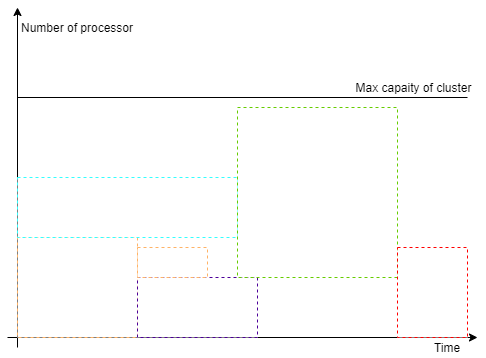
\includegraphics[width=\textwidth]{img/MPI_batch.png}
      \caption{Resources utilization of MPI batch jobs on cluster}
      \label{fig:MPI_batch}
  \end{subfigure}
  \begin{subfigure}[b]{0.45\textwidth}
      
\includegraphics[width=\textwidth]{img/spark_NP.png}
      \caption{Resources utilization of Spark on cluster}
      \label{fig:spark_np}
  \end{subfigure}
  \caption{The waste of compuation on cluster}\label{fig:waste_cluster}
\end{figure}
As it is shown in Fig. \ref{fig:MPI_batch}, MPI jobs are scheduled as fixed batch jobs which are colored boxes in the figure. It is very common to meet the situation that all jobs in the queue are too large and the number of idle resources is not enough for the jobs in the queue. 
For the Spark version, the possible situation can be visualized as Fig. \ref{sub@fig:spark_np}. The nodes should be reserved for Spark in advance and Spark task manager handles the task scheduling. For typical Spark applications relying on RDD, the number of required executors can be up and down dynamically. Part of computation resources may be wasted since this computation power is exclusive for Spark.
However, of course, the current Spark implementation for calibration is based on Driver mode and the granularity is one executor per task. In this case, the waste of resources won't happen within the Spark cluster. But when there are a lot of idle nodes in the cluster that not reserved for Spark at the beginning, they can not be used for Spark. 

In this project, we try to tackle on the issue of resource utilization. The LOFAR owns computation facility their own. Therefore, we take both perspectives of  cloud provider in Section 2 and cloud user in Section 3 into discussion.

\section{Cloud provider perspective}
The cloud providers own data centers with large quantity of and kinds of facilities. 
The resource management is the key point that the cloud provider will concern.
In 2013, Jennings and Stadler made a survey and listed challenges on Cloud resource management \cite{Jennings2015}.
They firstly lists actors in the cloud economy and then the fields of cloud technologies. 
Manvi and Shyam also made a survey on the same topic but it mainly focuses on IaaS cloud related aspects \cite{Manvi2014}. 
As it provides more observation from the technology side, the issues and definition of resource in clouds are given firstly.
In this section, the metrics around cloud are listed, as they are usually as the counterpart of resource utilization for trade off making.
And then, few related topics in the resource management field will be discussed.

\subsection{Metrics related to resource utilization}
In the cloud environment, there are many kinds of resources and a set of aspects around the cloud economy.
Both Jennings \cite{Jennings2015} and Manvi \cite{Manvi2014} starts with the definition of resources.

Jennings et al. categorize the resources into: compute, networking, storage, and power. 
Manvi at al. summarizes that there are physical resources(CPU,memory, storage, network elements and sensors ) and logical resources(OS, engergy, Network throughput/bandwidth,Load balancing mechanisms and so on).
There are overlap between two of them especially in the physical part, while Manvi adds API, OS, load balancing to logical resource concept.
However, it is understandable that API , OS and some protocols and mechanisms  can be viewed as some sort of asset of cloud owner, but they are more acceptable to be considered as part of Quality of Service(QoS) which needs resources to fulfill.
Therefore, in this section, we mainly focus on the utilization of physical resources like CPU, memory, storage; and consider the trade-off between utilization rate and QoS.

QoS (Quality of Service) metrics are import to both cloud provider and consumer, they are good for optimizing resource utilization efficiency
Bardsiri and Hashemi listed detailed metrics from four kinds of features:performance, economic, security and general. \cite{Bardsiri2014}
Their coverage is comprehensive. There are plenty of features and corresponding metrics that cloud users would put concern.

Given the background of researching utilization under limited resources, there are few metrics we consider important. 
For performance features, the CPU load rate and packet loss frequency are what users may concern while the cloud provides needs to make a compromise for utilization of resources.
In the economic aspect, the price per resource unit is the key point that cloud  providers and users wrestle on. However, from the technical view, the time for VM booting/deleting/suspending/provison attract more attantion.
Besides, the availability and reliability are very important. The response time is the key metric for auto-scaling mechanism.
Cloud providers need to pay effort on fault tolerance to make sure the safety of the cloud.

In the following sections, we will explore how cloud providers face resource management issues and the metrics shown above play important roles in  those researches.

\subsection{Resource demand profiling }
There is no doubt that before allocation and provision, it is vital to estimate the demanded resource of each workload. In this section, the workloads can be classified as two types: batch and interactive.
Different workload has different nature of their requirement of resources. 

For the batch applications, it is easier to estimate the resource demand. Given the parameters of each pre-identified application, the required resource over time can be calculated by a pre-trained model.
As an example, Becerra et al. purposed a methodology to profile the batch jobs. \cite{becerra2009batch} 
The workload profile is updated according  to the deviation  of CPU, memory, network usage by the time. 
% Besides of this typical approach, in Spark ecosystem, the resource demand can be calculated much more easier as each Spark batch job can be parsed to Directed Acyclic Graph(DAG) and the demanded resource in each state can be estimated.
% According to this feature, Databrick implements  auto-scaling mechanism\footnote{\url{https://databricks.com/blog/2018/05/02/introducing-databricks-optimized-auto-scaling.html}} within it the required resources can be dynamically calculated.

It is clear that the workload of web applications varies dynamically over multiple time scales.
section{Resource utilization optimization on Cloud/Cluster environment}
In this section, the definition of resource in the cloud field will be elaborated first, and the other important metrics that stakeholders concern.
Following the development path in this topic, a few kinds of approaches, and their typical examples will be explored.
Note that these approaches became popular one by one, but it does not mean the later ones are replacing previous ones.
The introduction of new technologies has led to the emergence of new methods and expanded the field's boundaries.
\subsection{Definition of resource and QoS}
There are many kinds of resources in the cloud environment and a set of aspects around the cloud economy.
Both Jennings \cite{Jennings2015} and Manvi \cite{Manvi2014} starts with the definition of resources.

Jennings et al. categorize the resources into computing, networking, storage, and power. 
Manvi et al. summarize that there are physical resources(CPU, memory, storage, network elements, and sensors ) and logical resources(OS, energy, Network throughput/bandwidth, Load balancing mechanisms, e.g.).
There is an overlap between the two of them, especially in the physical part, while Manvi adds API, OS, load balancing to the logical resource concept.
However, it is understandable that API, OS, and some protocols and mechanisms can be viewed as some assets of cloud owners, but they are more acceptable to be considered part of Quality of Service(QoS), which requires resources to fulfill.
Therefore, in this paper, we mainly focus on utilizing physical resources like CPU, memory, storage; and consider the trade-off between utilization rate and QoS.

QoS (Quality of Service) metrics are essential to both the cloud provider and the consumer; they are useful for optimizing resource utilization efficiency.
Bardsiri and Hashemi listed detailed metrics from four features: performance, economic, security, and general. \cite{Bardsiri2014}
Their coverage is comprehensive. There are plenty of features and corresponding metrics that cloud users would put concern.

Given the background of researching utilization under limited resources, there are few metrics we consider essential. 
For performance features, the CPU load rate and packet loss frequency are what users may concern, while the cloud provides needs to make a compromise for the utilization of resources.
The price per resource unit is the key point that cloud providers and users wrestle on in the economic aspect. However, the time for VM booting/deleting/suspending/provision attracts more attention from the technical view.
Besides, availability and reliability are crucial as well. The response time is the key metric for the auto-scaling mechanism.
Cloud providers need to pay effort on fault tolerance to make sure the safety of the cloud.

In the following sections, we will explore how cloud providers face resource management issues, and the metrics shown above play essential roles in those researches.

\subsection{Scheduling strategies on batch queuing systems }
The batch schedule has a long history in the entire computer science field, from the beginning of the mainframe age, and still part of the basic configuration of current research and systems.
The queuing system schedules jobs according to their priorities as the resource waste of FIFO is obvious. Therefore, A good deal of optimization is applied to the priorities related concepts.
Preemption, backfill, and heuristics are traditional routes for scheduling. Besides, with the growth of computation ability, the machine learning/deep learning approaches, which are based on historical data, become the forefront of research in this field.

Preemption is usually used to avoid job delaying and resources starvation. Furthermore, of course, the cost will be the re-do of preempted jobs. 
At the resources level, the preemption strategy is not common to be directly used on job scheduling along. Usually, it combines with other purposes.
For instance, Sajjapongse et al. \cite{sajjapongse2013preemption} designed a runtime system based on a preemption strategy to increase GPU utilization on heterogeneous clusters.
The performance of hybrid MPI-CUDA applications shows that preemption is an effective mechanism. 
To overcome the drawbacks, the resources waste, many adaptions are made. 
Lu Cheng et al. \cite{6103959} makes one of them for MapReduce. They introduced a component called Global Preemption to trade short-term fairness for better efficiency.
However, in the cloud/cluster environment, preemption strategies are used very carefully. Unless all jobs are equipped with a caching mechanism, the cost of canceling running jobs will be unaffordable.

The backfill algorithm is now the most common default schedule algorithm to achieve better resource utilization. 
This algorithm gives small jobs a higher priority to start first. The detail is explained in Section \ref{sec:backfill}.
However, of course, there is still a performance limit on this algorithm. 
Suresh et al. use a balanced spiral method applied to cloud metaschedules\cite{5972255}. It improves the performance and, at the same time, meets the requirement of QoS.
Nayak et al. proposed a novel backfilling-based task scheduling algorithm to schedule
deadline-based tasks\cite{nayak2019dynamic}. It aims to break the performance limit of the default backfilling algorithm of OpenNebula.
This VM based solution achieved decent resource utilization ascension.

Heuristics algorithms are usually more efficient, take less time to decide as scheduling problem is NP-Hard problem.
Xhafa and Abraham did a survey\cite{xhafa2010computational} and explored the appliance of heuristics algorithms on job scheduling. The most common and straightforward approach is local search.
Methods in this family include Hill Climbing (HC), Simulated Annealing (SA), and Tabu Search (TS), among others.
In \cite{ritchie2003fast}, local search helps schedule shortened on benchmark problems.
The population-based approaches are more efficient but require a longer time to convergence.
In \cite{abraham2000nature}, the Genetic Algorithm approach lets the resource entirely in use. 
Moreover, of course, in this work, the above two approaches are shown that they can be combined to have a better performance.  

In the last few years, the machine/deep learning has a big step of improvement. 
A very typical example is made by Mao et al. \cite{mao2016resource}, it shows (deep)reinforcement learning is able to achieve outperformance on traditional state-of-art approaches.
It translates the problem of packing tasks with multiple resources (here is CPU and memory) demands into a learning problem.
Another similar example\cite{8622393} also shows that the RL-based approach has great potential for resource management.
However, this work is not very convincing as the tested job arriving patterns are constructed via the Bernoulli process, Uniform distribution, and Beta distribution.
The real workload would not be easy to predict, and the patterns would not be simple as a specific distribution.
In other words, the performance should be measured on real workloads.


\subsection{Virtual machine founded cloud era}

After the first introduction by Eric Schmidt in 2006, cloud computing met its sharp increase.
The development of cloud computing is based on the maturation of virtualization technologies. 
The fine-granularity dividable resource enables users to obtain the 'pay-as-you-go' resources, and data centers can profit from selling every portion of the resource.

More detailed, the cloud users and cloud providers make a formal agreement known as SLA(Service level agreement).
Both cloud providers and cloud consumers need to formulate their management functions regarding the SLAs as for cloud consumers; they also need to meet the SLA requirement to their end-users.
Besides the SLAs, the data center infrastructure-related objectives include load-balancing, fault tolerance, and energy.
While for cloud users, they need to make a trade-off: conservative over-provisioning but less profit or aggressive minimizing cost but a higher risk of violating SLAs.
Considering the resources, computation, networking, storage, power, and etc., academia and industry developed mechanisms or systems to meet SLAs' requirements and achieve better resource management, thus more financially efficient. 

The most straightforward approach is to optimize the global scheduling of virtualized resources.
The core algorithms for the solution of virtual resource placement and provisioning has overlapped with the approaches in the previous section.
Mills et al. compared 18 (heuristics) VM placement algorithms by experiments and parameter grid search\cite{mills2011comparing} in 2011.
The 18 algorithms are made of a combination of 3 criteria for choosing a cluster, times six heuristics for choosing nodes under the two-level taxonomy.
The results reflect the no-free-lunch theorem in optimization: the percent-allocated (PAL) cluster-choice criterion leads to higher average loads and utilization, but this benefit of a cloud provider is based on the negative effect on users, for instance, the waiting time; 
Least-Full first(LF) and Tag\&Pack(TP) lead to lower cloud-wide virtual core utilization as these heuristics more often choose empty nodes on which to place VMs. However, LF  tends to squeeze out some larger VM types, which leads to yield lower user success rate and higher give-up rate.
This comparison gives a benchmark for cloud providers to determine which algorithm to employ. On the other hand, it indicates that the significant outperformance usually exists in the domain-specific scenario.
Recent researches support this trending. The \cite{moges2019energy} focuses on energy aware VM placement; the traffic linked placement solution is purposed in \cite{liwei2020online}; and \cite{kim2019holistic} considers the VM placement in heterogeneous clusters.

Following the VM placement, dynamic placement comes to the stage naturally, which benefits from the VM rescaling and live migration.
Sharma et al. \cite{5961733}\cite{5935016} formulated the problems of VM rescaling, replication and lived migration under the cost-efficient scenario as Integer Linear Programming problems
, and proposed Kingfisher, a set of techniques based on greedy heuristic solutions.
This work shows a cost-aware rescaling and lives migration algorithm can reduce the cost of VM transition(paused, serialized, and transferred to a different PM) compared to the cost-oblivious algorithms.
In \cite{6172596}, Wuhib et al. propose a decentralized solution, utilizing a gossip protocol. It is shown to scale to problem sizes above 150,000 PMs and 350,000 VMs and reduces the number of migrations.

Furthermore, the global scheduling for applications and VMs requires resource demand profiling, resource utilization estimation, and resource pricing \& profit maximization as a compliment.
For demand profiling, a typical model-based solution is \cite{gong2010press}, which employs Fast Fourier Transform(FFT) for resource usage detecting and a discrete-time Markov chain for demand predictions.
Furthermore, it was extended by online adaptive padding and reactive error correction to mitigate under-estimation\cite{shen2011cloudscale}.
Resource utilization estimation is not popular in research as the metrics for utilization are very clear.
The considerable research in this topic may relate to the special metric. 
For instance, in \cite{gmach2011chargeback}, a particular CPU and memory-related utilization metrics used by VMware’s Distributed Power Management (DPM) is discussed as it has effects on VMware’s power management mechanism.
In \cite{6847931}, Zhao et al. developed an online algorithm to maximize the profit of the cloud provider over the long run via scheduling job over data centers cross geolocation.

Following the global scheduling, the local scheduling of VM is vital as well.
The explicit solutions may formulate the problem into the allocation of physical machine resources to VMs.
Urgaonkar et al. proposed an approach aiming to dynamic resource allocation based on queuing information. Therefore the online control is achieve\cite{5488484}.
Each physical machine is equipped with a resource controller and a buffer(queue) containing applications in this approach.
Thus, as it is shown in the work \cite{6195591}, the sequence of the execution of VMs on PM has a significant impact on response time.
The authors propose a local scheduler combining both compute resource allocation and control of VM execution sequencing.

The researches mentioned above are collected due to their representative. Most of them are either published in the early 2010s or very recent.
Overall, these researches reflect a trend that after years of development in the cloud area, resource management research at the VM level has been to an in-depth and much more scenario dependent.
One remarkable exception is that with the rising of deep learning, the state-of-art on old and general topics has a big step forward.
The historical statistic based deep(reinforcement) learning models show substantial advantages on traditional rule-based, fuzzy theory, and heuristic solutions.

\subsection{Container and orchestra}
VMs enables clouds to achieve elasticity of large-scale shared resources, while it is still a heavyweight solution for dynamic provisioning.
Containers as a lightweight technology to virtualize applications have recently been successful and widely used for especially web applications.
Docker is the most popular container solution in the industry at this mount. Therefore, efficient management of the container layer, inserted between VMs and applications, is the must for a container-based cloud.
The management can be implemented directly or on top of container orchestras like Kubernetes or docker swarm.
Researches may either focus on direct management or the management with the help of orchestra frameworks.

The problems can be considered the same as resource management on VM; global scheduling is the most straightforward approach.
Due to the lightweight nature of containerization, the placement of containers can be more flexible.
In \cite{zhang2018container}, the authors proposed architecture for docker container placement.
It especially takes into consideration the collaboration of two kinds(container and VM) of placement.
Normally, The placements of the VM to PM and container to VM are based on the best-fit algorithm.
This work extends the best-fit algorithm, and the placement of containers should consider the resource utilization of PM.
However, this work considers the problem of container placement on VM as a bin pack problem. This assumption makes local scheduling of operating systems useless, and the elasticity of container has been sacrificed.
Another work\cite{7023588} is proposed for container placement as well, which is called Resource Stable Placement(RSP). The difference in architecture is that there is no VM placement problem, only the placement of containers on heterogeneous PMs.
The resources are modeled via a vector where each element represents the amount of one kind of resource.
Therefore, more than CPU and memory can be considered for resource placement.
This scheduling optimization shows better performance in response time and utilization of resources when the workload is heavy.

Besides the direct management, using the orchestra tool, especially like Kubernetes, are the most common approach.
In \cite{medel2016modelling}, the authors developed a Reference net-based model that employs real data from Kubernetes.
It characterizes the performance of Kubernetes and the lifecycle of containers and Pod. 
Kubernetes provides a diverse interface for task management and resource management.
However, as it is mentioned in \cite{wei2018research}, the scheduling only considers the current optimal node, regardless of the use of resource costs.
It provides a better allocation of  Pod scheduling, which is based on the Ant Colony Algorithm and Particle Swarm Algorithm.
The result of experiments on CloudSIM shows resource utilization, and load balancing can be improved significantly.


\newpage  
\bibliography{sample-base.bib}
\bibliographystyle{ACM-Reference-Format}

\end{document}
\endinput
%%
%% End of file `sample-sigchi.tex'.

